\documentclass[twoside]{book}

% Packages required by doxygen
\usepackage{fixltx2e}
\usepackage{calc}
\usepackage{doxygen}
\usepackage[export]{adjustbox} % also loads graphicx
\usepackage{graphicx}
\usepackage[utf8]{inputenc}
\usepackage{makeidx}
\usepackage{multicol}
\usepackage{multirow}
\PassOptionsToPackage{warn}{textcomp}
\usepackage{textcomp}
\usepackage[nointegrals]{wasysym}
\usepackage[table]{xcolor}

% Font selection
\usepackage[T1]{fontenc}
\usepackage[scaled=.90]{helvet}
\usepackage{courier}
\usepackage{amssymb}
\usepackage{sectsty}
\renewcommand{\familydefault}{\sfdefault}
\allsectionsfont{%
  \fontseries{bc}\selectfont%
  \color{darkgray}%
}
\renewcommand{\DoxyLabelFont}{%
  \fontseries{bc}\selectfont%
  \color{darkgray}%
}
\newcommand{\+}{\discretionary{\mbox{\scriptsize$\hookleftarrow$}}{}{}}

% Page & text layout
\usepackage{geometry}
\geometry{%
  a4paper,%
  top=2.5cm,%
  bottom=2.5cm,%
  left=2.5cm,%
  right=2.5cm%
}
\tolerance=750
\hfuzz=15pt
\hbadness=750
\setlength{\emergencystretch}{15pt}
\setlength{\parindent}{0cm}
\setlength{\parskip}{3ex plus 2ex minus 2ex}
\makeatletter
\renewcommand{\paragraph}{%
  \@startsection{paragraph}{4}{0ex}{-1.0ex}{1.0ex}{%
    \normalfont\normalsize\bfseries\SS@parafont%
  }%
}
\renewcommand{\subparagraph}{%
  \@startsection{subparagraph}{5}{0ex}{-1.0ex}{1.0ex}{%
    \normalfont\normalsize\bfseries\SS@subparafont%
  }%
}
\makeatother

% Headers & footers
\usepackage{fancyhdr}
\pagestyle{fancyplain}
\fancyhead[LE]{\fancyplain{}{\bfseries\thepage}}
\fancyhead[CE]{\fancyplain{}{}}
\fancyhead[RE]{\fancyplain{}{\bfseries\leftmark}}
\fancyhead[LO]{\fancyplain{}{\bfseries\rightmark}}
\fancyhead[CO]{\fancyplain{}{}}
\fancyhead[RO]{\fancyplain{}{\bfseries\thepage}}
\fancyfoot[LE]{\fancyplain{}{}}
\fancyfoot[CE]{\fancyplain{}{}}
\fancyfoot[RE]{\fancyplain{}{\bfseries\scriptsize Generated by Doxygen }}
\fancyfoot[LO]{\fancyplain{}{\bfseries\scriptsize Generated by Doxygen }}
\fancyfoot[CO]{\fancyplain{}{}}
\fancyfoot[RO]{\fancyplain{}{}}
\renewcommand{\footrulewidth}{0.4pt}
\renewcommand{\chaptermark}[1]{%
  \markboth{#1}{}%
}
\renewcommand{\sectionmark}[1]{%
  \markright{\thesection\ #1}%
}

% Indices & bibliography
\usepackage{natbib}
\usepackage[titles]{tocloft}
\setcounter{tocdepth}{3}
\setcounter{secnumdepth}{5}
\makeindex

% Hyperlinks (required, but should be loaded last)
\usepackage{ifpdf}
\ifpdf
  \usepackage[pdftex,pagebackref=true]{hyperref}
\else
  \usepackage[ps2pdf,pagebackref=true]{hyperref}
\fi
\hypersetup{%
  colorlinks=true,%
  linkcolor=blue,%
  citecolor=blue,%
  unicode%
}

% Custom commands
\newcommand{\clearemptydoublepage}{%
  \newpage{\pagestyle{empty}\cleardoublepage}%
}

\usepackage{caption}
\captionsetup{labelsep=space,justification=centering,font={bf},singlelinecheck=off,skip=4pt,position=top}

%===== C O N T E N T S =====

\begin{document}

% Titlepage & ToC
\hypersetup{pageanchor=false,
             bookmarksnumbered=true,
             pdfencoding=unicode
            }
\pagenumbering{alph}
\begin{titlepage}
\vspace*{7cm}
\begin{center}%
{\Large personage principal }\\
\vspace*{1cm}
{\large Generated by Doxygen 1.8.13}\\
\end{center}
\end{titlepage}
\clearemptydoublepage
\pagenumbering{roman}
\tableofcontents
\clearemptydoublepage
\pagenumbering{arabic}
\hypersetup{pageanchor=true}

%--- Begin generated contents ---
\chapter{Data Structure Index}
\section{Data Structures}
Here are the data structures with brief descriptions\+:\begin{DoxyCompactList}
\item\contentsline{section}{\hyperlink{structLife}{Life} \\*Structure pour l\textquotesingle{}affichage les vies du joueur }{\pageref{structLife}}{}
\item\contentsline{section}{\hyperlink{structPersonnage__Principal}{Personnage\+\_\+\+Principal} \\*Structure pour le personnage principal }{\pageref{structPersonnage__Principal}}{}
\item\contentsline{section}{\hyperlink{structScore}{Score} \\*Structure pour l\textquotesingle{}affichage du score }{\pageref{structScore}}{}
\end{DoxyCompactList}

\chapter{File Index}
\section{File List}
Here is a list of all files with brief descriptions\+:\begin{DoxyCompactList}
\item\contentsline{section}{\hyperlink{main_8c}{main.\+c} \\*Tester le programme }{\pageref{main_8c}}{}
\item\contentsline{section}{\hyperlink{PP_8c}{P\+P.\+c} \\*Fonction of the main charactere }{\pageref{PP_8c}}{}
\item\contentsline{section}{\hyperlink{PP_8h}{P\+P.\+h} \\*Headers and strctures }{\pageref{PP_8h}}{}
\end{DoxyCompactList}

\chapter{Data Structure Documentation}
\hypertarget{structLife}{}\section{Life Struct Reference}
\label{structLife}\index{Life@{Life}}


structure pour l\textquotesingle{}affichage les vies du joueur  




{\ttfamily \#include $<$P\+P.\+h$>$}

\subsection*{Data Fields}
\begin{DoxyCompactItemize}
\item 
int \hyperlink{structLife_acf338f9197d398ce4e796accbde75266}{Nbr\+\_\+\+Life}
\item 
S\+D\+L\+\_\+\+Surface $\ast$ \hyperlink{structLife_a019e5fa5af83a0e1ecb5de0a09540f19}{Life\+\_\+img}
\item 
S\+D\+L\+\_\+\+Rect \hyperlink{structLife_ac23b346f3b87e8259cd5766521ee3f01}{Position\+\_\+life}
\end{DoxyCompactItemize}


\subsection{Detailed Description}
structure pour l\textquotesingle{}affichage les vies du joueur 

\subsection{Field Documentation}
\mbox{\Hypertarget{structLife_a019e5fa5af83a0e1ecb5de0a09540f19}\label{structLife_a019e5fa5af83a0e1ecb5de0a09540f19}} 
\index{Life@{Life}!Life\+\_\+img@{Life\+\_\+img}}
\index{Life\+\_\+img@{Life\+\_\+img}!Life@{Life}}
\subsubsection{\texorpdfstring{Life\+\_\+img}{Life\_img}}
{\footnotesize\ttfamily S\+D\+L\+\_\+\+Surface$\ast$ Life\+::\+Life\+\_\+img}

la variable S\+D\+L\+\_\+\+Surface des vies \mbox{\Hypertarget{structLife_acf338f9197d398ce4e796accbde75266}\label{structLife_acf338f9197d398ce4e796accbde75266}} 
\index{Life@{Life}!Nbr\+\_\+\+Life@{Nbr\+\_\+\+Life}}
\index{Nbr\+\_\+\+Life@{Nbr\+\_\+\+Life}!Life@{Life}}
\subsubsection{\texorpdfstring{Nbr\+\_\+\+Life}{Nbr\_Life}}
{\footnotesize\ttfamily int Life\+::\+Nbr\+\_\+\+Life}

nombre de vie restant au joueur \mbox{\Hypertarget{structLife_ac23b346f3b87e8259cd5766521ee3f01}\label{structLife_ac23b346f3b87e8259cd5766521ee3f01}} 
\index{Life@{Life}!Position\+\_\+life@{Position\+\_\+life}}
\index{Position\+\_\+life@{Position\+\_\+life}!Life@{Life}}
\subsubsection{\texorpdfstring{Position\+\_\+life}{Position\_life}}
{\footnotesize\ttfamily S\+D\+L\+\_\+\+Rect Life\+::\+Position\+\_\+life}

position des vies de joueur 

The documentation for this struct was generated from the following file\+:\begin{DoxyCompactItemize}
\item 
\hyperlink{PP_8h}{P\+P.\+h}\end{DoxyCompactItemize}

\hypertarget{structPersonnage__Principal}{}\section{Personnage\+\_\+\+Principal Struct Reference}
\label{structPersonnage__Principal}\index{Personnage\+\_\+\+Principal@{Personnage\+\_\+\+Principal}}


structure pour le personnage principal  




{\ttfamily \#include $<$P\+P.\+h$>$}



Collaboration diagram for Personnage\+\_\+\+Principal\+:\nopagebreak
\begin{figure}[H]
\begin{center}
\leavevmode
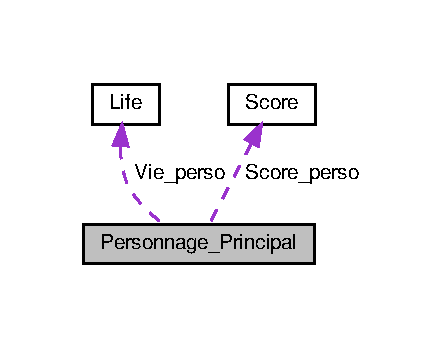
\includegraphics[width=213pt]{structPersonnage__Principal__coll__graph}
\end{center}
\end{figure}
\subsection*{Data Fields}
\begin{DoxyCompactItemize}
\item 
S\+D\+L\+\_\+\+Surface $\ast$ \hyperlink{structPersonnage__Principal_a9ae86c3cfc13f35afabffac632cd9274}{Sprite\+\_\+sheet}
\item 
S\+D\+L\+\_\+\+Rect \hyperlink{structPersonnage__Principal_a1d3adc7ba5a683c3170addb0be59414f}{Position\+\_\+intiale}
\item 
S\+D\+L\+\_\+\+Rect \hyperlink{structPersonnage__Principal_aae3f91b7533eaff379444b2a099cdabc}{Pos\+\_\+\+Sprite}
\item 
\hyperlink{structLife}{Life} \hyperlink{structPersonnage__Principal_a5d7356f35759733b870eab1f598bcd2e}{Vie\+\_\+perso}
\item 
\hyperlink{structScore}{Score} \hyperlink{structPersonnage__Principal_a92c56f66fbf10945b1ed7ed3163c6c99}{Score\+\_\+perso}
\item 
int \hyperlink{structPersonnage__Principal_ab1859deae3c17ed820bd9c2eb2a67f00}{limite\+\_\+min}
\item 
int \hyperlink{structPersonnage__Principal_a096c666c96d412155d978951abcd4691}{limite\+\_\+max}
\item 
int \hyperlink{structPersonnage__Principal_a2a4fd91e82c16257be3b3675bcf4fc8f}{Direction}
\item 
int \hyperlink{structPersonnage__Principal_a2a942d64b6c4affbbd7917f7d83724d4}{Mouvement}
\item 
int \hyperlink{structPersonnage__Principal_aa94e2bfad60dee47da88d7862e9dbb1b}{acceleration}
\item 
int \hyperlink{structPersonnage__Principal_aacb52649fa0a8f0e822d03837ce3ed83}{max\+\_\+frame}
\item 
int \hyperlink{structPersonnage__Principal_aee6abfc2eb74dd9aceb9437b6b734bc2}{frame}
\item 
int \hyperlink{structPersonnage__Principal_a4dd6ca03003b960b83689e04fb30c43a}{jump}
\end{DoxyCompactItemize}


\subsection{Detailed Description}
structure pour le personnage principal 

\subsection{Field Documentation}
\mbox{\Hypertarget{structPersonnage__Principal_aa94e2bfad60dee47da88d7862e9dbb1b}\label{structPersonnage__Principal_aa94e2bfad60dee47da88d7862e9dbb1b}} 
\index{Personnage\+\_\+\+Principal@{Personnage\+\_\+\+Principal}!acceleration@{acceleration}}
\index{acceleration@{acceleration}!Personnage\+\_\+\+Principal@{Personnage\+\_\+\+Principal}}
\subsubsection{\texorpdfstring{acceleration}{acceleration}}
{\footnotesize\ttfamily int Personnage\+\_\+\+Principal\+::acceleration}

confession d\textquotesingle{}acceleration \mbox{\Hypertarget{structPersonnage__Principal_a2a4fd91e82c16257be3b3675bcf4fc8f}\label{structPersonnage__Principal_a2a4fd91e82c16257be3b3675bcf4fc8f}} 
\index{Personnage\+\_\+\+Principal@{Personnage\+\_\+\+Principal}!Direction@{Direction}}
\index{Direction@{Direction}!Personnage\+\_\+\+Principal@{Personnage\+\_\+\+Principal}}
\subsubsection{\texorpdfstring{Direction}{Direction}}
{\footnotesize\ttfamily int Personnage\+\_\+\+Principal\+::\+Direction}

la variable de direction 1 a droit 2 a gauche \mbox{\Hypertarget{structPersonnage__Principal_aee6abfc2eb74dd9aceb9437b6b734bc2}\label{structPersonnage__Principal_aee6abfc2eb74dd9aceb9437b6b734bc2}} 
\index{Personnage\+\_\+\+Principal@{Personnage\+\_\+\+Principal}!frame@{frame}}
\index{frame@{frame}!Personnage\+\_\+\+Principal@{Personnage\+\_\+\+Principal}}
\subsubsection{\texorpdfstring{frame}{frame}}
{\footnotesize\ttfamily int Personnage\+\_\+\+Principal\+::frame}

le frame actuel du personnage \mbox{\Hypertarget{structPersonnage__Principal_a4dd6ca03003b960b83689e04fb30c43a}\label{structPersonnage__Principal_a4dd6ca03003b960b83689e04fb30c43a}} 
\index{Personnage\+\_\+\+Principal@{Personnage\+\_\+\+Principal}!jump@{jump}}
\index{jump@{jump}!Personnage\+\_\+\+Principal@{Personnage\+\_\+\+Principal}}
\subsubsection{\texorpdfstring{jump}{jump}}
{\footnotesize\ttfamily int Personnage\+\_\+\+Principal\+::jump}

la variable du saut 1 ou 0 \mbox{\Hypertarget{structPersonnage__Principal_a096c666c96d412155d978951abcd4691}\label{structPersonnage__Principal_a096c666c96d412155d978951abcd4691}} 
\index{Personnage\+\_\+\+Principal@{Personnage\+\_\+\+Principal}!limite\+\_\+max@{limite\+\_\+max}}
\index{limite\+\_\+max@{limite\+\_\+max}!Personnage\+\_\+\+Principal@{Personnage\+\_\+\+Principal}}
\subsubsection{\texorpdfstring{limite\+\_\+max}{limite\_max}}
{\footnotesize\ttfamily int Personnage\+\_\+\+Principal\+::limite\+\_\+max}

la limit a droite du mouvement du personnage \mbox{\Hypertarget{structPersonnage__Principal_ab1859deae3c17ed820bd9c2eb2a67f00}\label{structPersonnage__Principal_ab1859deae3c17ed820bd9c2eb2a67f00}} 
\index{Personnage\+\_\+\+Principal@{Personnage\+\_\+\+Principal}!limite\+\_\+min@{limite\+\_\+min}}
\index{limite\+\_\+min@{limite\+\_\+min}!Personnage\+\_\+\+Principal@{Personnage\+\_\+\+Principal}}
\subsubsection{\texorpdfstring{limite\+\_\+min}{limite\_min}}
{\footnotesize\ttfamily int Personnage\+\_\+\+Principal\+::limite\+\_\+min}

la limit a gauche du mouvement du personnage \mbox{\Hypertarget{structPersonnage__Principal_aacb52649fa0a8f0e822d03837ce3ed83}\label{structPersonnage__Principal_aacb52649fa0a8f0e822d03837ce3ed83}} 
\index{Personnage\+\_\+\+Principal@{Personnage\+\_\+\+Principal}!max\+\_\+frame@{max\+\_\+frame}}
\index{max\+\_\+frame@{max\+\_\+frame}!Personnage\+\_\+\+Principal@{Personnage\+\_\+\+Principal}}
\subsubsection{\texorpdfstring{max\+\_\+frame}{max\_frame}}
{\footnotesize\ttfamily int Personnage\+\_\+\+Principal\+::max\+\_\+frame}

max frame du personnage dans le spritsheet \mbox{\Hypertarget{structPersonnage__Principal_a2a942d64b6c4affbbd7917f7d83724d4}\label{structPersonnage__Principal_a2a942d64b6c4affbbd7917f7d83724d4}} 
\index{Personnage\+\_\+\+Principal@{Personnage\+\_\+\+Principal}!Mouvement@{Mouvement}}
\index{Mouvement@{Mouvement}!Personnage\+\_\+\+Principal@{Personnage\+\_\+\+Principal}}
\subsubsection{\texorpdfstring{Mouvement}{Mouvement}}
{\footnotesize\ttfamily int Personnage\+\_\+\+Principal\+::\+Mouvement}

le type de mouvement du personnage \mbox{\Hypertarget{structPersonnage__Principal_aae3f91b7533eaff379444b2a099cdabc}\label{structPersonnage__Principal_aae3f91b7533eaff379444b2a099cdabc}} 
\index{Personnage\+\_\+\+Principal@{Personnage\+\_\+\+Principal}!Pos\+\_\+\+Sprite@{Pos\+\_\+\+Sprite}}
\index{Pos\+\_\+\+Sprite@{Pos\+\_\+\+Sprite}!Personnage\+\_\+\+Principal@{Personnage\+\_\+\+Principal}}
\subsubsection{\texorpdfstring{Pos\+\_\+\+Sprite}{Pos\_Sprite}}
{\footnotesize\ttfamily S\+D\+L\+\_\+\+Rect Personnage\+\_\+\+Principal\+::\+Pos\+\_\+\+Sprite}

la position du frame actuelle dans le spritesheet \mbox{\Hypertarget{structPersonnage__Principal_a1d3adc7ba5a683c3170addb0be59414f}\label{structPersonnage__Principal_a1d3adc7ba5a683c3170addb0be59414f}} 
\index{Personnage\+\_\+\+Principal@{Personnage\+\_\+\+Principal}!Position\+\_\+intiale@{Position\+\_\+intiale}}
\index{Position\+\_\+intiale@{Position\+\_\+intiale}!Personnage\+\_\+\+Principal@{Personnage\+\_\+\+Principal}}
\subsubsection{\texorpdfstring{Position\+\_\+intiale}{Position\_intiale}}
{\footnotesize\ttfamily S\+D\+L\+\_\+\+Rect Personnage\+\_\+\+Principal\+::\+Position\+\_\+intiale}

position du personage \mbox{\Hypertarget{structPersonnage__Principal_a92c56f66fbf10945b1ed7ed3163c6c99}\label{structPersonnage__Principal_a92c56f66fbf10945b1ed7ed3163c6c99}} 
\index{Personnage\+\_\+\+Principal@{Personnage\+\_\+\+Principal}!Score\+\_\+perso@{Score\+\_\+perso}}
\index{Score\+\_\+perso@{Score\+\_\+perso}!Personnage\+\_\+\+Principal@{Personnage\+\_\+\+Principal}}
\subsubsection{\texorpdfstring{Score\+\_\+perso}{Score\_perso}}
{\footnotesize\ttfamily \hyperlink{structScore}{Score} Personnage\+\_\+\+Principal\+::\+Score\+\_\+perso}

score du personnage \mbox{\Hypertarget{structPersonnage__Principal_a9ae86c3cfc13f35afabffac632cd9274}\label{structPersonnage__Principal_a9ae86c3cfc13f35afabffac632cd9274}} 
\index{Personnage\+\_\+\+Principal@{Personnage\+\_\+\+Principal}!Sprite\+\_\+sheet@{Sprite\+\_\+sheet}}
\index{Sprite\+\_\+sheet@{Sprite\+\_\+sheet}!Personnage\+\_\+\+Principal@{Personnage\+\_\+\+Principal}}
\subsubsection{\texorpdfstring{Sprite\+\_\+sheet}{Sprite\_sheet}}
{\footnotesize\ttfamily S\+D\+L\+\_\+\+Surface$\ast$ Personnage\+\_\+\+Principal\+::\+Sprite\+\_\+sheet}

la variabel S\+D\+L\+\_\+\+Surface du spritesheet du personnage \mbox{\Hypertarget{structPersonnage__Principal_a5d7356f35759733b870eab1f598bcd2e}\label{structPersonnage__Principal_a5d7356f35759733b870eab1f598bcd2e}} 
\index{Personnage\+\_\+\+Principal@{Personnage\+\_\+\+Principal}!Vie\+\_\+perso@{Vie\+\_\+perso}}
\index{Vie\+\_\+perso@{Vie\+\_\+perso}!Personnage\+\_\+\+Principal@{Personnage\+\_\+\+Principal}}
\subsubsection{\texorpdfstring{Vie\+\_\+perso}{Vie\_perso}}
{\footnotesize\ttfamily \hyperlink{structLife}{Life} Personnage\+\_\+\+Principal\+::\+Vie\+\_\+perso}

les vies du personnage 

The documentation for this struct was generated from the following file\+:\begin{DoxyCompactItemize}
\item 
\hyperlink{PP_8h}{P\+P.\+h}\end{DoxyCompactItemize}

\hypertarget{structScore}{}\section{Score Struct Reference}
\label{structScore}\index{Score@{Score}}


structure pour l\textquotesingle{}affichage du score  




{\ttfamily \#include $<$P\+P.\+h$>$}

\subsection*{Data Fields}
\begin{DoxyCompactItemize}
\item 
S\+D\+L\+\_\+\+Surface $\ast$ \hyperlink{structScore_aa1e07a19fbd1cb60bd7358b64ffac283}{Score}
\item 
S\+D\+L\+\_\+\+Rect \hyperlink{structScore_a8402710c14fc3b01a15b4c324844705e}{Position\+\_\+score}
\item 
int \hyperlink{structScore_a34dd585c0a3fd0b39ac754e072ee1476}{S}
\end{DoxyCompactItemize}


\subsection{Detailed Description}
structure pour l\textquotesingle{}affichage du score 

\subsection{Field Documentation}
\mbox{\Hypertarget{structScore_a8402710c14fc3b01a15b4c324844705e}\label{structScore_a8402710c14fc3b01a15b4c324844705e}} 
\index{Score@{Score}!Position\+\_\+score@{Position\+\_\+score}}
\index{Position\+\_\+score@{Position\+\_\+score}!Score@{Score}}
\subsubsection{\texorpdfstring{Position\+\_\+score}{Position\_score}}
{\footnotesize\ttfamily S\+D\+L\+\_\+\+Rect Score\+::\+Position\+\_\+score}

la position du score dans l\textquotesingle{}ecran \mbox{\Hypertarget{structScore_a34dd585c0a3fd0b39ac754e072ee1476}\label{structScore_a34dd585c0a3fd0b39ac754e072ee1476}} 
\index{Score@{Score}!S@{S}}
\index{S@{S}!Score@{Score}}
\subsubsection{\texorpdfstring{S}{S}}
{\footnotesize\ttfamily int Score\+::S}

la valeur du score du joueur \mbox{\Hypertarget{structScore_aa1e07a19fbd1cb60bd7358b64ffac283}\label{structScore_aa1e07a19fbd1cb60bd7358b64ffac283}} 
\index{Score@{Score}!Score@{Score}}
\index{Score@{Score}!Score@{Score}}
\subsubsection{\texorpdfstring{Score}{Score}}
{\footnotesize\ttfamily S\+D\+L\+\_\+\+Surface$\ast$ Score\+::\+Score}

la variable S\+D\+L\+\_\+\+Surface du score 

The documentation for this struct was generated from the following file\+:\begin{DoxyCompactItemize}
\item 
\hyperlink{PP_8h}{P\+P.\+h}\end{DoxyCompactItemize}

\chapter{File Documentation}
\hypertarget{main_8c}{}\section{main.\+c File Reference}
\label{main_8c}\index{main.\+c@{main.\+c}}


tester le programme  


{\ttfamily \#include $<$S\+D\+L/\+S\+D\+L.\+h$>$}\newline
{\ttfamily \#include $<$S\+D\+L/\+S\+D\+L\+\_\+image.\+h$>$}\newline
{\ttfamily \#include $<$S\+D\+L/\+S\+D\+L\+\_\+mixer.\+h$>$}\newline
{\ttfamily \#include $<$S\+D\+L/\+S\+D\+L\+\_\+ttf.\+h$>$}\newline
{\ttfamily \#include $<$stdlib.\+h$>$}\newline
{\ttfamily \#include $<$stdio.\+h$>$}\newline
{\ttfamily \#include \char`\"{}P\+P.\+h\char`\"{}}\newline
Include dependency graph for main.\+c\+:\nopagebreak
\begin{figure}[H]
\begin{center}
\leavevmode
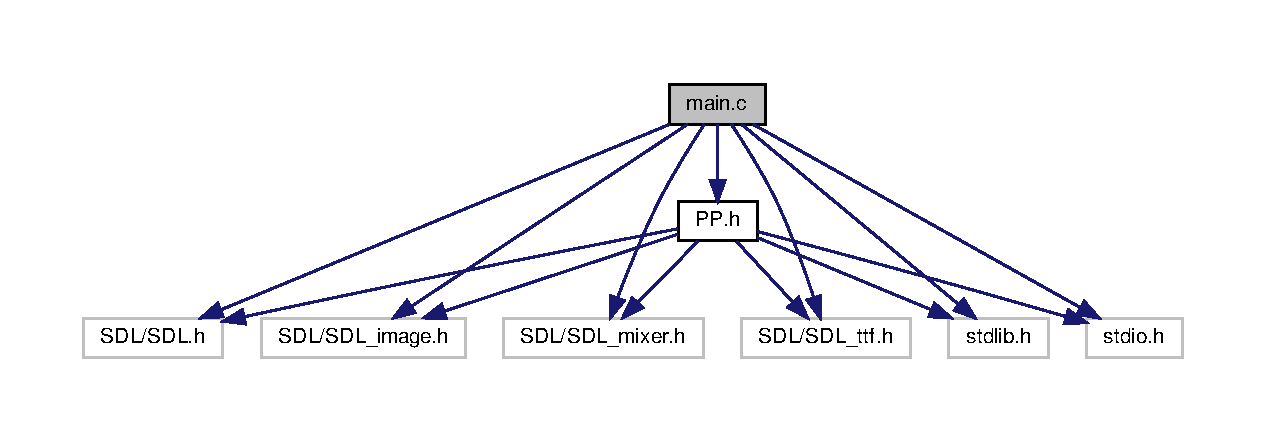
\includegraphics[width=350pt]{main_8c__incl}
\end{center}
\end{figure}
\subsection*{Macros}
\begin{DoxyCompactItemize}
\item 
\#define \hyperlink{main_8c_ac292291c26a5202c8e3cf749bca7daf6}{x\+\_\+screen\+\_\+size}~1150
\item 
\#define \hyperlink{main_8c_a6c322d2ad52f03717c4dcaac088beba4}{y\+\_\+screen\+\_\+size}~914
\item 
\#define \hyperlink{main_8c_af613cadd5cf49515a2b8790d3bfd56af}{mode}~0
\end{DoxyCompactItemize}
\subsection*{Functions}
\begin{DoxyCompactItemize}
\item 
int \hyperlink{main_8c_ae66f6b31b5ad750f1fe042a706a4e3d4}{main} ()
\end{DoxyCompactItemize}


\subsection{Detailed Description}
tester le programme 

\begin{DoxyAuthor}{Author}
haythem jaidane 
\end{DoxyAuthor}
\begin{DoxyVersion}{Version}
0.\+6 
\end{DoxyVersion}
\begin{DoxyDate}{Date}
Apr 20, 2021 
\end{DoxyDate}


\subsection{Macro Definition Documentation}
\mbox{\Hypertarget{main_8c_af613cadd5cf49515a2b8790d3bfd56af}\label{main_8c_af613cadd5cf49515a2b8790d3bfd56af}} 
\index{main.\+c@{main.\+c}!mode@{mode}}
\index{mode@{mode}!main.\+c@{main.\+c}}
\subsubsection{\texorpdfstring{mode}{mode}}
{\footnotesize\ttfamily \#define mode~0}

\mbox{\Hypertarget{main_8c_ac292291c26a5202c8e3cf749bca7daf6}\label{main_8c_ac292291c26a5202c8e3cf749bca7daf6}} 
\index{main.\+c@{main.\+c}!x\+\_\+screen\+\_\+size@{x\+\_\+screen\+\_\+size}}
\index{x\+\_\+screen\+\_\+size@{x\+\_\+screen\+\_\+size}!main.\+c@{main.\+c}}
\subsubsection{\texorpdfstring{x\+\_\+screen\+\_\+size}{x\_screen\_size}}
{\footnotesize\ttfamily \#define x\+\_\+screen\+\_\+size~1150}

\mbox{\Hypertarget{main_8c_a6c322d2ad52f03717c4dcaac088beba4}\label{main_8c_a6c322d2ad52f03717c4dcaac088beba4}} 
\index{main.\+c@{main.\+c}!y\+\_\+screen\+\_\+size@{y\+\_\+screen\+\_\+size}}
\index{y\+\_\+screen\+\_\+size@{y\+\_\+screen\+\_\+size}!main.\+c@{main.\+c}}
\subsubsection{\texorpdfstring{y\+\_\+screen\+\_\+size}{y\_screen\_size}}
{\footnotesize\ttfamily \#define y\+\_\+screen\+\_\+size~914}



\subsection{Function Documentation}
\mbox{\Hypertarget{main_8c_ae66f6b31b5ad750f1fe042a706a4e3d4}\label{main_8c_ae66f6b31b5ad750f1fe042a706a4e3d4}} 
\index{main.\+c@{main.\+c}!main@{main}}
\index{main@{main}!main.\+c@{main.\+c}}
\subsubsection{\texorpdfstring{main()}{main()}}
{\footnotesize\ttfamily int main (\begin{DoxyParamCaption}{ }\end{DoxyParamCaption})}

Here is the call graph for this function\+:\nopagebreak
\begin{figure}[H]
\begin{center}
\leavevmode
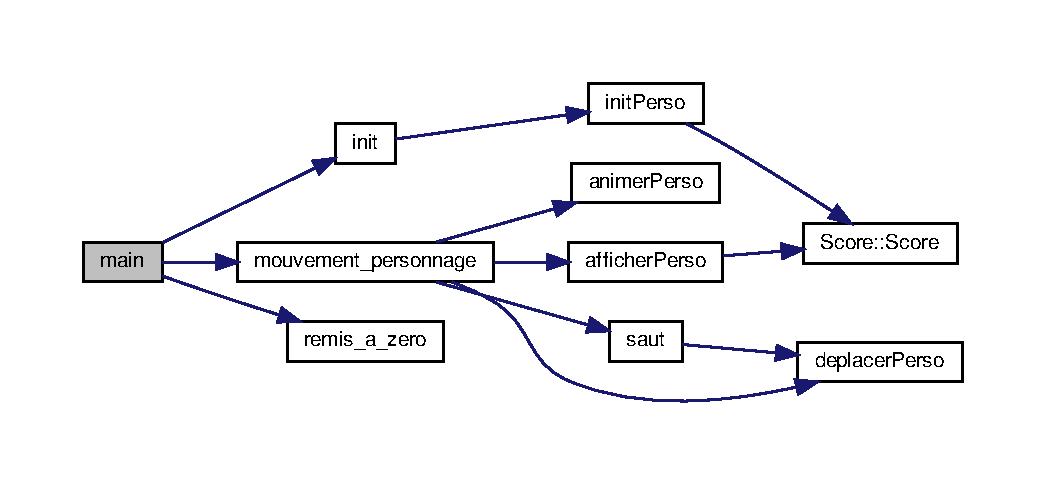
\includegraphics[width=350pt]{main_8c_ae66f6b31b5ad750f1fe042a706a4e3d4_cgraph}
\end{center}
\end{figure}

\hypertarget{PP_8c}{}\section{P\+P.\+c File Reference}
\label{PP_8c}\index{P\+P.\+c@{P\+P.\+c}}


fonction of the main charactere  


{\ttfamily \#include $<$S\+D\+L/\+S\+D\+L.\+h$>$}\newline
{\ttfamily \#include $<$S\+D\+L/\+S\+D\+L\+\_\+image.\+h$>$}\newline
{\ttfamily \#include $<$S\+D\+L/\+S\+D\+L\+\_\+mixer.\+h$>$}\newline
{\ttfamily \#include $<$S\+D\+L/\+S\+D\+L\+\_\+ttf.\+h$>$}\newline
{\ttfamily \#include $<$stdlib.\+h$>$}\newline
{\ttfamily \#include $<$stdio.\+h$>$}\newline
{\ttfamily \#include $<$string.\+h$>$}\newline
{\ttfamily \#include \char`\"{}P\+P.\+h\char`\"{}}\newline
Include dependency graph for P\+P.\+c\+:
\nopagebreak
\begin{figure}[H]
\begin{center}
\leavevmode
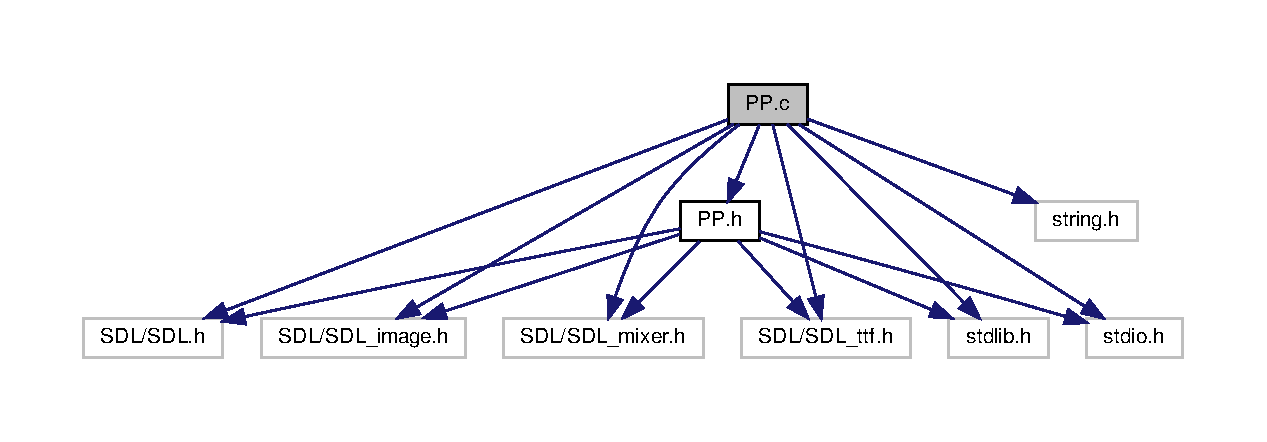
\includegraphics[width=350pt]{PP_8c__incl}
\end{center}
\end{figure}
\subsection*{Functions}
\begin{DoxyCompactItemize}
\item 
void \hyperlink{PP_8c_a06d4dad62654fc7399c91ef52e319c3c}{init\+Perso} (\hyperlink{structPersonnage__Principal}{Personnage\+\_\+\+Principal} $\ast$p)
\begin{DoxyCompactList}\small\item\em pour initialisier un personnage principal ( cette fonction est inisialiser sur le Spritesheet de test ) \end{DoxyCompactList}\item 
void \hyperlink{PP_8c_a929664b87fb6288f8e2eb696a0bd2ccb}{init} (\hyperlink{structPersonnage__Principal}{Personnage\+\_\+\+Principal} tab\+\_\+p\mbox{[}$\,$\mbox{]}, int \hyperlink{main_8c_af613cadd5cf49515a2b8790d3bfd56af}{mode})
\begin{DoxyCompactList}\small\item\em pour initialisier le mode de jeu (single ou multiplayer) on initialise la position initial, les vies et le score de chaque charactere \end{DoxyCompactList}\item 
void \hyperlink{PP_8c_a742fd43f3d683af543f04032cc7bf6d0}{afficher\+Perso} (\hyperlink{structPersonnage__Principal}{Personnage\+\_\+\+Principal} p, S\+D\+L\+\_\+\+Surface $\ast$screen)
\begin{DoxyCompactList}\small\item\em pour afficher le peronnage , les vies et le score sans screen flip . \end{DoxyCompactList}\item 
void \hyperlink{PP_8c_a208324da218a8c45e7b72520166b910d}{deplacer\+Perso} (\hyperlink{structPersonnage__Principal}{Personnage\+\_\+\+Principal} $\ast$p)
\begin{DoxyCompactList}\small\item\em pour deplacer le personnage principal . \end{DoxyCompactList}\item 
void \hyperlink{PP_8c_afc7631c9f2e3b0445fb7250a3dd6ddeb}{animer\+Perso} (\hyperlink{structPersonnage__Principal}{Personnage\+\_\+\+Principal} $\ast$p)
\begin{DoxyCompactList}\small\item\em pour animer le personnage principal en deplacent frame par frame. \end{DoxyCompactList}\item 
void \hyperlink{PP_8c_a23102f7e1f31031abb303525289bfb37}{saut} (\hyperlink{structPersonnage__Principal}{Personnage\+\_\+\+Principal} $\ast$p)
\begin{DoxyCompactList}\small\item\em pour faire sauter le peronnage ( cette fonction est faite pour un saut de 5 frame ). \end{DoxyCompactList}\item 
void \hyperlink{PP_8c_a9e39e2d357f18982e3ec80e8ee8e2401}{mouvement\+\_\+personnage} (\hyperlink{structPersonnage__Principal}{Personnage\+\_\+\+Principal} tab\+\_\+p\mbox{[}$\,$\mbox{]}, S\+D\+L\+\_\+\+Surface $\ast$screen, S\+D\+L\+\_\+\+Surface $\ast$background, S\+D\+L\+\_\+\+Rect position\+\_\+bakcground, int \hyperlink{main_8c_af613cadd5cf49515a2b8790d3bfd56af}{mode})
\begin{DoxyCompactList}\small\item\em pour faire le controle du personnage. \end{DoxyCompactList}\item 
void \hyperlink{PP_8c_a3fe04c57396598b16d78bd4065a8824d}{remis\+\_\+a\+\_\+zero} (\hyperlink{structPersonnage__Principal}{Personnage\+\_\+\+Principal} tab\+\_\+p\mbox{[}$\,$\mbox{]}, int \hyperlink{main_8c_af613cadd5cf49515a2b8790d3bfd56af}{mode})
\begin{DoxyCompactList}\small\item\em pour remettre a zero tout les paramettre du jeu apres boucle de jeu. \end{DoxyCompactList}\end{DoxyCompactItemize}


\subsection{Detailed Description}
fonction of the main charactere 

\begin{DoxyAuthor}{Author}
haythem jaidane 
\end{DoxyAuthor}
\begin{DoxyVersion}{Version}
0.\+6 
\end{DoxyVersion}
\begin{DoxyDate}{Date}
Apr 20, 2021 
\end{DoxyDate}


\subsection{Function Documentation}
\mbox{\Hypertarget{PP_8c_a742fd43f3d683af543f04032cc7bf6d0}\label{PP_8c_a742fd43f3d683af543f04032cc7bf6d0}} 
\index{P\+P.\+c@{P\+P.\+c}!afficher\+Perso@{afficher\+Perso}}
\index{afficher\+Perso@{afficher\+Perso}!P\+P.\+c@{P\+P.\+c}}
\subsubsection{\texorpdfstring{afficher\+Perso()}{afficherPerso()}}
{\footnotesize\ttfamily void afficher\+Perso (\begin{DoxyParamCaption}\item[{\hyperlink{structPersonnage__Principal}{Personnage\+\_\+\+Principal}}]{p,  }\item[{S\+D\+L\+\_\+\+Surface $\ast$}]{screen }\end{DoxyParamCaption})}



pour afficher le peronnage , les vies et le score sans screen flip . 


\begin{DoxyParams}{Parameters}
{\em p} & la variable du personnage \\
\hline
{\em screen} & la variable de l\textquotesingle{}ecran \\
\hline
\end{DoxyParams}
\begin{DoxyReturn}{Returns}
Nothing 
\end{DoxyReturn}
Here is the call graph for this function\+:
\nopagebreak
\begin{figure}[H]
\begin{center}
\leavevmode
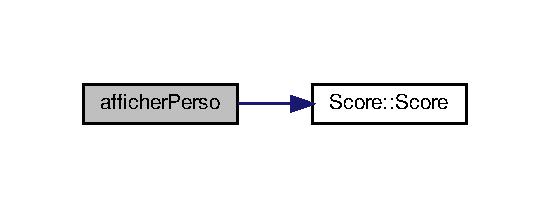
\includegraphics[width=264pt]{PP_8c_a742fd43f3d683af543f04032cc7bf6d0_cgraph}
\end{center}
\end{figure}
Here is the caller graph for this function\+:
\nopagebreak
\begin{figure}[H]
\begin{center}
\leavevmode
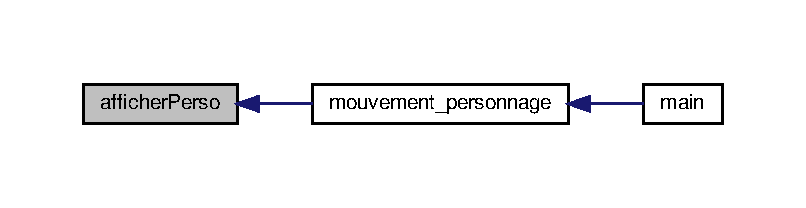
\includegraphics[width=350pt]{PP_8c_a742fd43f3d683af543f04032cc7bf6d0_icgraph}
\end{center}
\end{figure}
\mbox{\Hypertarget{PP_8c_afc7631c9f2e3b0445fb7250a3dd6ddeb}\label{PP_8c_afc7631c9f2e3b0445fb7250a3dd6ddeb}} 
\index{P\+P.\+c@{P\+P.\+c}!animer\+Perso@{animer\+Perso}}
\index{animer\+Perso@{animer\+Perso}!P\+P.\+c@{P\+P.\+c}}
\subsubsection{\texorpdfstring{animer\+Perso()}{animerPerso()}}
{\footnotesize\ttfamily void animer\+Perso (\begin{DoxyParamCaption}\item[{\hyperlink{structPersonnage__Principal}{Personnage\+\_\+\+Principal} $\ast$}]{p }\end{DoxyParamCaption})}



pour animer le personnage principal en deplacent frame par frame. 


\begin{DoxyParams}{Parameters}
{\em p} & la variable du personnage \\
\hline
\end{DoxyParams}
\begin{DoxyReturn}{Returns}
Nothing 
\end{DoxyReturn}
Here is the caller graph for this function\+:
\nopagebreak
\begin{figure}[H]
\begin{center}
\leavevmode
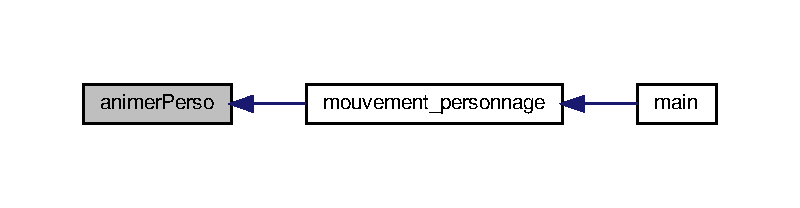
\includegraphics[width=350pt]{PP_8c_afc7631c9f2e3b0445fb7250a3dd6ddeb_icgraph}
\end{center}
\end{figure}
\mbox{\Hypertarget{PP_8c_a208324da218a8c45e7b72520166b910d}\label{PP_8c_a208324da218a8c45e7b72520166b910d}} 
\index{P\+P.\+c@{P\+P.\+c}!deplacer\+Perso@{deplacer\+Perso}}
\index{deplacer\+Perso@{deplacer\+Perso}!P\+P.\+c@{P\+P.\+c}}
\subsubsection{\texorpdfstring{deplacer\+Perso()}{deplacerPerso()}}
{\footnotesize\ttfamily void deplacer\+Perso (\begin{DoxyParamCaption}\item[{\hyperlink{structPersonnage__Principal}{Personnage\+\_\+\+Principal} $\ast$}]{p }\end{DoxyParamCaption})}



pour deplacer le personnage principal . 


\begin{DoxyParams}{Parameters}
{\em p} & la variable du personnage \\
\hline
\end{DoxyParams}
\begin{DoxyReturn}{Returns}
Nothing 
\end{DoxyReturn}
Here is the caller graph for this function\+:
\nopagebreak
\begin{figure}[H]
\begin{center}
\leavevmode
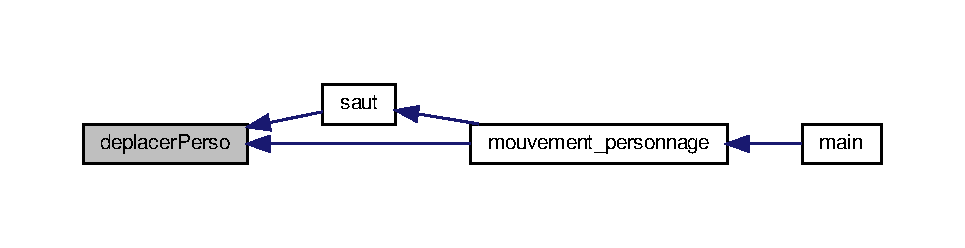
\includegraphics[width=350pt]{PP_8c_a208324da218a8c45e7b72520166b910d_icgraph}
\end{center}
\end{figure}
\mbox{\Hypertarget{PP_8c_a929664b87fb6288f8e2eb696a0bd2ccb}\label{PP_8c_a929664b87fb6288f8e2eb696a0bd2ccb}} 
\index{P\+P.\+c@{P\+P.\+c}!init@{init}}
\index{init@{init}!P\+P.\+c@{P\+P.\+c}}
\subsubsection{\texorpdfstring{init()}{init()}}
{\footnotesize\ttfamily void init (\begin{DoxyParamCaption}\item[{\hyperlink{structPersonnage__Principal}{Personnage\+\_\+\+Principal}}]{tab\+\_\+p\mbox{[}$\,$\mbox{]},  }\item[{int}]{mode }\end{DoxyParamCaption})}



pour initialisier le mode de jeu (single ou multiplayer) on initialise la position initial, les vies et le score de chaque charactere 


\begin{DoxyParams}{Parameters}
{\em tab\+\_\+p} & un tableau de 2 personnage \\
\hline
{\em mode} & 0 pour le mode singleplayer et 1 pour le mode multiplayer \\
\hline
\end{DoxyParams}
\begin{DoxyReturn}{Returns}
Nothing 
\end{DoxyReturn}
Here is the call graph for this function\+:
\nopagebreak
\begin{figure}[H]
\begin{center}
\leavevmode
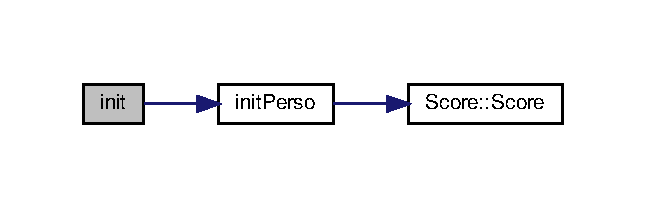
\includegraphics[width=310pt]{PP_8c_a929664b87fb6288f8e2eb696a0bd2ccb_cgraph}
\end{center}
\end{figure}
Here is the caller graph for this function\+:
\nopagebreak
\begin{figure}[H]
\begin{center}
\leavevmode
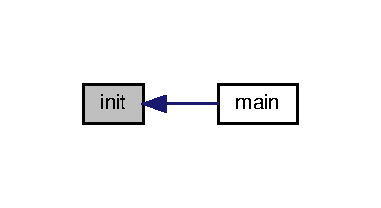
\includegraphics[width=183pt]{PP_8c_a929664b87fb6288f8e2eb696a0bd2ccb_icgraph}
\end{center}
\end{figure}
\mbox{\Hypertarget{PP_8c_a06d4dad62654fc7399c91ef52e319c3c}\label{PP_8c_a06d4dad62654fc7399c91ef52e319c3c}} 
\index{P\+P.\+c@{P\+P.\+c}!init\+Perso@{init\+Perso}}
\index{init\+Perso@{init\+Perso}!P\+P.\+c@{P\+P.\+c}}
\subsubsection{\texorpdfstring{init\+Perso()}{initPerso()}}
{\footnotesize\ttfamily void init\+Perso (\begin{DoxyParamCaption}\item[{\hyperlink{structPersonnage__Principal}{Personnage\+\_\+\+Principal} $\ast$}]{p }\end{DoxyParamCaption})}



pour initialisier un personnage principal ( cette fonction est inisialiser sur le Spritesheet de test ) 


\begin{DoxyParams}{Parameters}
{\em tab\+\_\+p} & un tableau de 2 personnage \\
\hline
\end{DoxyParams}
\begin{DoxyReturn}{Returns}
Nothing 
\end{DoxyReturn}
Here is the call graph for this function\+:
\nopagebreak
\begin{figure}[H]
\begin{center}
\leavevmode
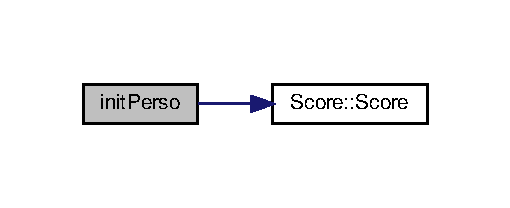
\includegraphics[width=245pt]{PP_8c_a06d4dad62654fc7399c91ef52e319c3c_cgraph}
\end{center}
\end{figure}
Here is the caller graph for this function\+:
\nopagebreak
\begin{figure}[H]
\begin{center}
\leavevmode
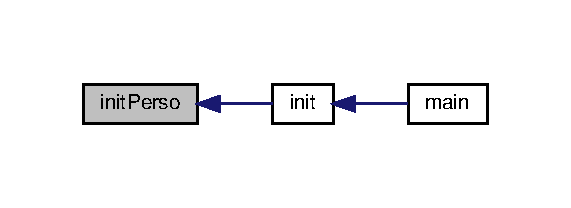
\includegraphics[width=274pt]{PP_8c_a06d4dad62654fc7399c91ef52e319c3c_icgraph}
\end{center}
\end{figure}
\mbox{\Hypertarget{PP_8c_a9e39e2d357f18982e3ec80e8ee8e2401}\label{PP_8c_a9e39e2d357f18982e3ec80e8ee8e2401}} 
\index{P\+P.\+c@{P\+P.\+c}!mouvement\+\_\+personnage@{mouvement\+\_\+personnage}}
\index{mouvement\+\_\+personnage@{mouvement\+\_\+personnage}!P\+P.\+c@{P\+P.\+c}}
\subsubsection{\texorpdfstring{mouvement\+\_\+personnage()}{mouvement\_personnage()}}
{\footnotesize\ttfamily void mouvement\+\_\+personnage (\begin{DoxyParamCaption}\item[{\hyperlink{structPersonnage__Principal}{Personnage\+\_\+\+Principal}}]{tab\+\_\+p\mbox{[}$\,$\mbox{]},  }\item[{S\+D\+L\+\_\+\+Surface $\ast$}]{screen,  }\item[{S\+D\+L\+\_\+\+Surface $\ast$}]{background,  }\item[{S\+D\+L\+\_\+\+Rect}]{position\+\_\+bakcground,  }\item[{int}]{mode }\end{DoxyParamCaption})}



pour faire le controle du personnage. 


\begin{DoxyParams}{Parameters}
{\em tab\+\_\+p} & un tableau de 2 personnage \\
\hline
{\em screen} & variable S\+D\+L\+\_\+\+Surface de l\textquotesingle{}ecran \\
\hline
{\em background} & variable S\+D\+L\+\_\+\+Surface du background \\
\hline
{\em position\+\_\+bakcground} & variable S\+D\+L\+\_\+\+Rect de la position du background \\
\hline
{\em mode} & 0 pour le mode singleplayer et 1 pour le mode multiplayer \\
\hline
\end{DoxyParams}
\begin{DoxyReturn}{Returns}
Nothing 
\end{DoxyReturn}
Here is the call graph for this function\+:
\nopagebreak
\begin{figure}[H]
\begin{center}
\leavevmode
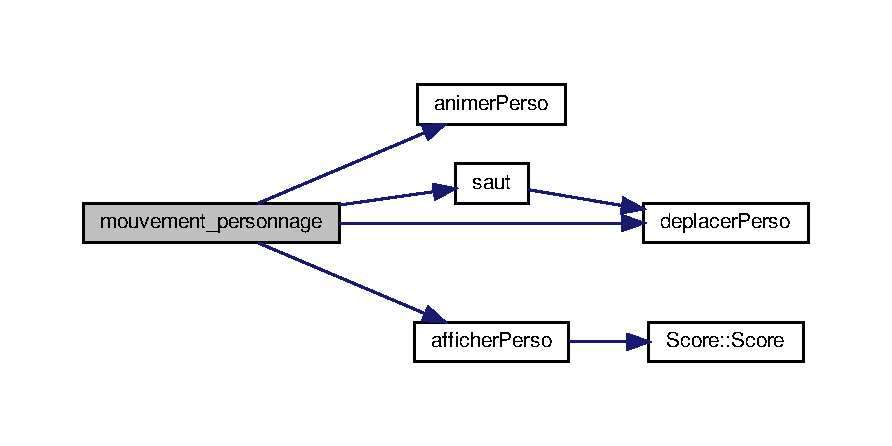
\includegraphics[width=350pt]{PP_8c_a9e39e2d357f18982e3ec80e8ee8e2401_cgraph}
\end{center}
\end{figure}
Here is the caller graph for this function\+:
\nopagebreak
\begin{figure}[H]
\begin{center}
\leavevmode
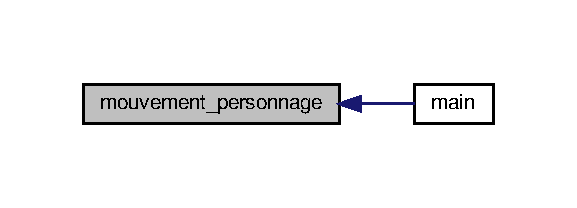
\includegraphics[width=277pt]{PP_8c_a9e39e2d357f18982e3ec80e8ee8e2401_icgraph}
\end{center}
\end{figure}
\mbox{\Hypertarget{PP_8c_a3fe04c57396598b16d78bd4065a8824d}\label{PP_8c_a3fe04c57396598b16d78bd4065a8824d}} 
\index{P\+P.\+c@{P\+P.\+c}!remis\+\_\+a\+\_\+zero@{remis\+\_\+a\+\_\+zero}}
\index{remis\+\_\+a\+\_\+zero@{remis\+\_\+a\+\_\+zero}!P\+P.\+c@{P\+P.\+c}}
\subsubsection{\texorpdfstring{remis\+\_\+a\+\_\+zero()}{remis\_a\_zero()}}
{\footnotesize\ttfamily void remis\+\_\+a\+\_\+zero (\begin{DoxyParamCaption}\item[{\hyperlink{structPersonnage__Principal}{Personnage\+\_\+\+Principal}}]{tab\+\_\+p\mbox{[}$\,$\mbox{]},  }\item[{int}]{mode }\end{DoxyParamCaption})}



pour remettre a zero tout les paramettre du jeu apres boucle de jeu. 


\begin{DoxyParams}{Parameters}
{\em tab\+\_\+p} & un tableau de 2 personnage \\
\hline
{\em mode} & 0 pour le mode singleplayer et 1 pour le mode multiplayer \\
\hline
\end{DoxyParams}
\begin{DoxyReturn}{Returns}
Nothing 
\end{DoxyReturn}
Here is the caller graph for this function\+:
\nopagebreak
\begin{figure}[H]
\begin{center}
\leavevmode
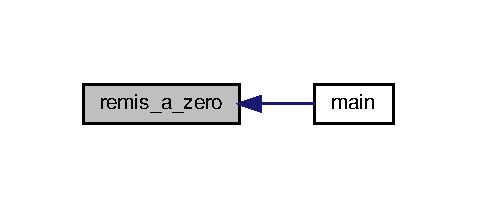
\includegraphics[width=229pt]{PP_8c_a3fe04c57396598b16d78bd4065a8824d_icgraph}
\end{center}
\end{figure}
\mbox{\Hypertarget{PP_8c_a23102f7e1f31031abb303525289bfb37}\label{PP_8c_a23102f7e1f31031abb303525289bfb37}} 
\index{P\+P.\+c@{P\+P.\+c}!saut@{saut}}
\index{saut@{saut}!P\+P.\+c@{P\+P.\+c}}
\subsubsection{\texorpdfstring{saut()}{saut()}}
{\footnotesize\ttfamily void saut (\begin{DoxyParamCaption}\item[{\hyperlink{structPersonnage__Principal}{Personnage\+\_\+\+Principal} $\ast$}]{p }\end{DoxyParamCaption})}



pour faire sauter le peronnage ( cette fonction est faite pour un saut de 5 frame ). 


\begin{DoxyParams}{Parameters}
{\em p} & la variable du personnage \\
\hline
\end{DoxyParams}
\begin{DoxyReturn}{Returns}
Nothing 
\end{DoxyReturn}
Here is the call graph for this function\+:
\nopagebreak
\begin{figure}[H]
\begin{center}
\leavevmode
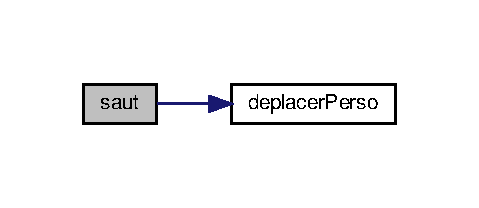
\includegraphics[width=230pt]{PP_8c_a23102f7e1f31031abb303525289bfb37_cgraph}
\end{center}
\end{figure}
Here is the caller graph for this function\+:
\nopagebreak
\begin{figure}[H]
\begin{center}
\leavevmode
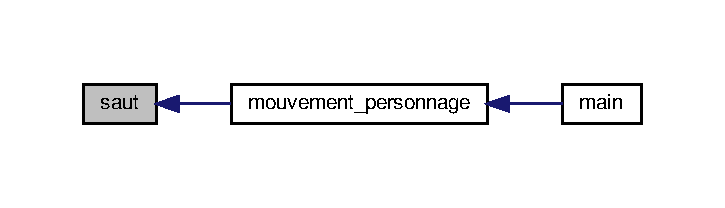
\includegraphics[width=348pt]{PP_8c_a23102f7e1f31031abb303525289bfb37_icgraph}
\end{center}
\end{figure}

\hypertarget{PP_8h}{}\section{P\+P.\+h File Reference}
\label{PP_8h}\index{P\+P.\+h@{P\+P.\+h}}


headers and strctures  


{\ttfamily \#include $<$S\+D\+L/\+S\+D\+L.\+h$>$}\newline
{\ttfamily \#include $<$stdio.\+h$>$}\newline
{\ttfamily \#include $<$stdlib.\+h$>$}\newline
{\ttfamily \#include $<$S\+D\+L/\+S\+D\+L\+\_\+image.\+h$>$}\newline
{\ttfamily \#include $<$S\+D\+L/\+S\+D\+L\+\_\+mixer.\+h$>$}\newline
{\ttfamily \#include $<$S\+D\+L/\+S\+D\+L\+\_\+ttf.\+h$>$}\newline
Include dependency graph for P\+P.\+h\+:\nopagebreak
\begin{figure}[H]
\begin{center}
\leavevmode
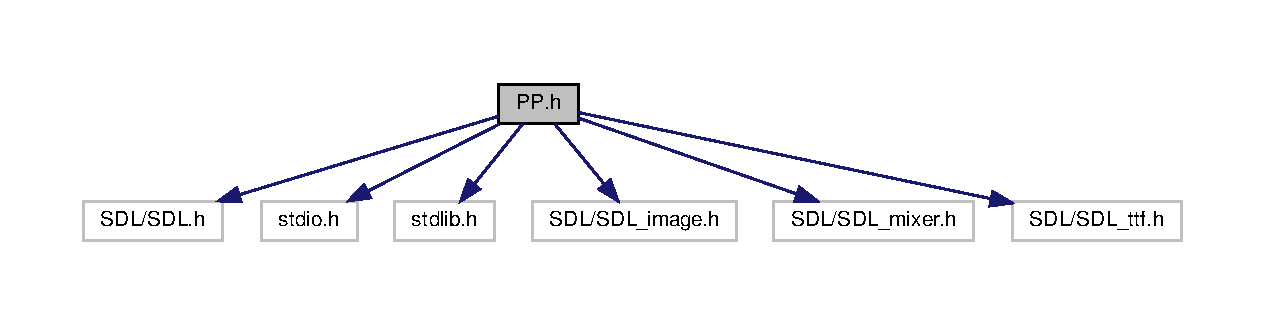
\includegraphics[width=350pt]{PP_8h__incl}
\end{center}
\end{figure}
This graph shows which files directly or indirectly include this file\+:\nopagebreak
\begin{figure}[H]
\begin{center}
\leavevmode
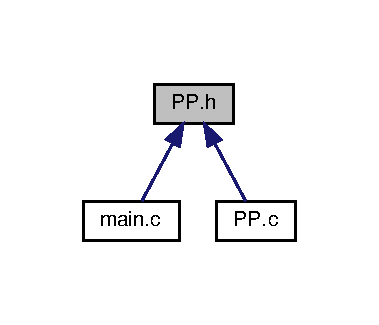
\includegraphics[width=182pt]{PP_8h__dep__incl}
\end{center}
\end{figure}
\subsection*{Data Structures}
\begin{DoxyCompactItemize}
\item 
struct \hyperlink{structLife}{Life}
\begin{DoxyCompactList}\small\item\em structure pour l\textquotesingle{}affichage les vies du joueur \end{DoxyCompactList}\item 
struct \hyperlink{structScore}{Score}
\begin{DoxyCompactList}\small\item\em structure pour l\textquotesingle{}affichage du score \end{DoxyCompactList}\item 
struct \hyperlink{structPersonnage__Principal}{Personnage\+\_\+\+Principal}
\begin{DoxyCompactList}\small\item\em structure pour le personnage principal \end{DoxyCompactList}\end{DoxyCompactItemize}
\subsection*{Functions}
\begin{DoxyCompactItemize}
\item 
void \hyperlink{PP_8h_a06d4dad62654fc7399c91ef52e319c3c}{init\+Perso} (\hyperlink{structPersonnage__Principal}{Personnage\+\_\+\+Principal} $\ast$p)
\begin{DoxyCompactList}\small\item\em pour initialisier un personnage principal ( cette fonction est inisialiser sur le Spritesheet de test ) \end{DoxyCompactList}\item 
void \hyperlink{PP_8h_a929664b87fb6288f8e2eb696a0bd2ccb}{init} (\hyperlink{structPersonnage__Principal}{Personnage\+\_\+\+Principal} tab\+\_\+p\mbox{[}$\,$\mbox{]}, int \hyperlink{main_8c_af613cadd5cf49515a2b8790d3bfd56af}{mode})
\begin{DoxyCompactList}\small\item\em pour initialisier le mode de jeu (single ou multiplayer) on initialise la position initial, les vies et le score de chaque charactere \end{DoxyCompactList}\item 
void \hyperlink{PP_8h_a742fd43f3d683af543f04032cc7bf6d0}{afficher\+Perso} (\hyperlink{structPersonnage__Principal}{Personnage\+\_\+\+Principal} p, S\+D\+L\+\_\+\+Surface $\ast$screen)
\begin{DoxyCompactList}\small\item\em pour afficher le peronnage , les vies et le score sans screen flip . \end{DoxyCompactList}\item 
void \hyperlink{PP_8h_a208324da218a8c45e7b72520166b910d}{deplacer\+Perso} (\hyperlink{structPersonnage__Principal}{Personnage\+\_\+\+Principal} $\ast$p)
\begin{DoxyCompactList}\small\item\em pour deplacer le personnage principal . \end{DoxyCompactList}\item 
void \hyperlink{PP_8h_afc7631c9f2e3b0445fb7250a3dd6ddeb}{animer\+Perso} (\hyperlink{structPersonnage__Principal}{Personnage\+\_\+\+Principal} $\ast$p)
\begin{DoxyCompactList}\small\item\em pour animer le personnage principal en deplacent frame par frame. \end{DoxyCompactList}\item 
void \hyperlink{PP_8h_a23102f7e1f31031abb303525289bfb37}{saut} (\hyperlink{structPersonnage__Principal}{Personnage\+\_\+\+Principal} $\ast$p)
\begin{DoxyCompactList}\small\item\em pour faire sauter le peronnage ( cette fonction est faite pour un saut de 5 frame ). \end{DoxyCompactList}\item 
void \hyperlink{PP_8h_a9e39e2d357f18982e3ec80e8ee8e2401}{mouvement\+\_\+personnage} (\hyperlink{structPersonnage__Principal}{Personnage\+\_\+\+Principal} tab\+\_\+p\mbox{[}$\,$\mbox{]}, S\+D\+L\+\_\+\+Surface $\ast$screen, S\+D\+L\+\_\+\+Surface $\ast$background, S\+D\+L\+\_\+\+Rect position\+\_\+bakcground, int \hyperlink{main_8c_af613cadd5cf49515a2b8790d3bfd56af}{mode})
\begin{DoxyCompactList}\small\item\em pour faire le controle du personnage. \end{DoxyCompactList}\item 
void \hyperlink{PP_8h_a3fe04c57396598b16d78bd4065a8824d}{remis\+\_\+a\+\_\+zero} (\hyperlink{structPersonnage__Principal}{Personnage\+\_\+\+Principal} tab\+\_\+p\mbox{[}$\,$\mbox{]}, int \hyperlink{main_8c_af613cadd5cf49515a2b8790d3bfd56af}{mode})
\begin{DoxyCompactList}\small\item\em pour remettre a zero tout les paramettre du jeu apres boucle de jeu. \end{DoxyCompactList}\end{DoxyCompactItemize}


\subsection{Detailed Description}
headers and strctures 

\begin{DoxyAuthor}{Author}
haythem jaidane 
\end{DoxyAuthor}
\begin{DoxyVersion}{Version}
0.\+6 
\end{DoxyVersion}
\begin{DoxyDate}{Date}
Apr 20, 2021 
\end{DoxyDate}


\subsection{Function Documentation}
\mbox{\Hypertarget{PP_8h_a742fd43f3d683af543f04032cc7bf6d0}\label{PP_8h_a742fd43f3d683af543f04032cc7bf6d0}} 
\index{P\+P.\+h@{P\+P.\+h}!afficher\+Perso@{afficher\+Perso}}
\index{afficher\+Perso@{afficher\+Perso}!P\+P.\+h@{P\+P.\+h}}
\subsubsection{\texorpdfstring{afficher\+Perso()}{afficherPerso()}}
{\footnotesize\ttfamily void afficher\+Perso (\begin{DoxyParamCaption}\item[{\hyperlink{structPersonnage__Principal}{Personnage\+\_\+\+Principal}}]{p,  }\item[{S\+D\+L\+\_\+\+Surface $\ast$}]{screen }\end{DoxyParamCaption})}



pour afficher le peronnage , les vies et le score sans screen flip . 


\begin{DoxyParams}{Parameters}
{\em p} & la variable du personnage \\
\hline
{\em screen} & la variable de l\textquotesingle{}ecran \\
\hline
\end{DoxyParams}
\begin{DoxyReturn}{Returns}
Nothing 
\end{DoxyReturn}
Here is the call graph for this function\+:\nopagebreak
\begin{figure}[H]
\begin{center}
\leavevmode
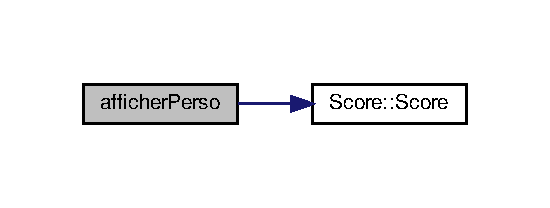
\includegraphics[width=264pt]{PP_8h_a742fd43f3d683af543f04032cc7bf6d0_cgraph}
\end{center}
\end{figure}
Here is the caller graph for this function\+:\nopagebreak
\begin{figure}[H]
\begin{center}
\leavevmode
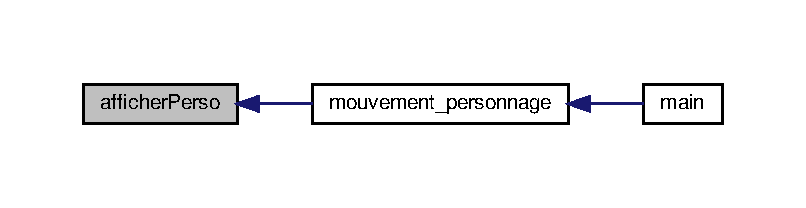
\includegraphics[width=350pt]{PP_8h_a742fd43f3d683af543f04032cc7bf6d0_icgraph}
\end{center}
\end{figure}
\mbox{\Hypertarget{PP_8h_afc7631c9f2e3b0445fb7250a3dd6ddeb}\label{PP_8h_afc7631c9f2e3b0445fb7250a3dd6ddeb}} 
\index{P\+P.\+h@{P\+P.\+h}!animer\+Perso@{animer\+Perso}}
\index{animer\+Perso@{animer\+Perso}!P\+P.\+h@{P\+P.\+h}}
\subsubsection{\texorpdfstring{animer\+Perso()}{animerPerso()}}
{\footnotesize\ttfamily void animer\+Perso (\begin{DoxyParamCaption}\item[{\hyperlink{structPersonnage__Principal}{Personnage\+\_\+\+Principal} $\ast$}]{p }\end{DoxyParamCaption})}



pour animer le personnage principal en deplacent frame par frame. 


\begin{DoxyParams}{Parameters}
{\em p} & la variable du personnage \\
\hline
\end{DoxyParams}
\begin{DoxyReturn}{Returns}
Nothing 
\end{DoxyReturn}
Here is the caller graph for this function\+:\nopagebreak
\begin{figure}[H]
\begin{center}
\leavevmode
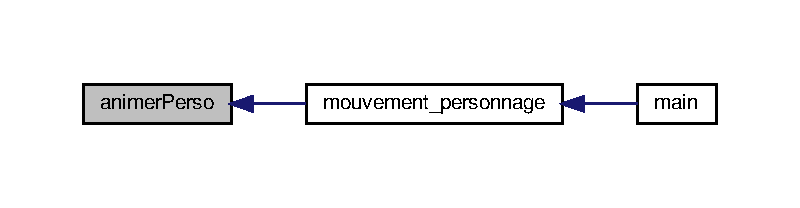
\includegraphics[width=350pt]{PP_8h_afc7631c9f2e3b0445fb7250a3dd6ddeb_icgraph}
\end{center}
\end{figure}
\mbox{\Hypertarget{PP_8h_a208324da218a8c45e7b72520166b910d}\label{PP_8h_a208324da218a8c45e7b72520166b910d}} 
\index{P\+P.\+h@{P\+P.\+h}!deplacer\+Perso@{deplacer\+Perso}}
\index{deplacer\+Perso@{deplacer\+Perso}!P\+P.\+h@{P\+P.\+h}}
\subsubsection{\texorpdfstring{deplacer\+Perso()}{deplacerPerso()}}
{\footnotesize\ttfamily void deplacer\+Perso (\begin{DoxyParamCaption}\item[{\hyperlink{structPersonnage__Principal}{Personnage\+\_\+\+Principal} $\ast$}]{p }\end{DoxyParamCaption})}



pour deplacer le personnage principal . 


\begin{DoxyParams}{Parameters}
{\em p} & la variable du personnage \\
\hline
\end{DoxyParams}
\begin{DoxyReturn}{Returns}
Nothing 
\end{DoxyReturn}
Here is the caller graph for this function\+:\nopagebreak
\begin{figure}[H]
\begin{center}
\leavevmode
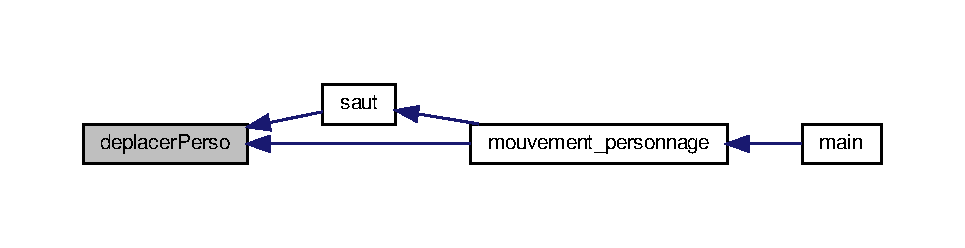
\includegraphics[width=350pt]{PP_8h_a208324da218a8c45e7b72520166b910d_icgraph}
\end{center}
\end{figure}
\mbox{\Hypertarget{PP_8h_a929664b87fb6288f8e2eb696a0bd2ccb}\label{PP_8h_a929664b87fb6288f8e2eb696a0bd2ccb}} 
\index{P\+P.\+h@{P\+P.\+h}!init@{init}}
\index{init@{init}!P\+P.\+h@{P\+P.\+h}}
\subsubsection{\texorpdfstring{init()}{init()}}
{\footnotesize\ttfamily void init (\begin{DoxyParamCaption}\item[{\hyperlink{structPersonnage__Principal}{Personnage\+\_\+\+Principal}}]{tab\+\_\+p\mbox{[}$\,$\mbox{]},  }\item[{int}]{mode }\end{DoxyParamCaption})}



pour initialisier le mode de jeu (single ou multiplayer) on initialise la position initial, les vies et le score de chaque charactere 


\begin{DoxyParams}{Parameters}
{\em tab\+\_\+p} & un tableau de 2 personnage \\
\hline
{\em mode} & 0 pour le mode singleplayer et 1 pour le mode multiplayer \\
\hline
\end{DoxyParams}
\begin{DoxyReturn}{Returns}
Nothing 
\end{DoxyReturn}
Here is the call graph for this function\+:\nopagebreak
\begin{figure}[H]
\begin{center}
\leavevmode
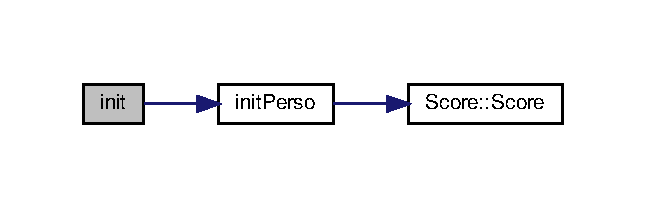
\includegraphics[width=310pt]{PP_8h_a929664b87fb6288f8e2eb696a0bd2ccb_cgraph}
\end{center}
\end{figure}
Here is the caller graph for this function\+:\nopagebreak
\begin{figure}[H]
\begin{center}
\leavevmode
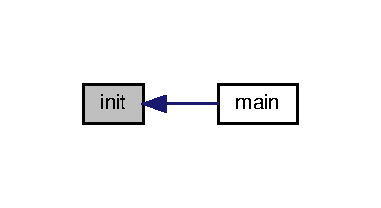
\includegraphics[width=183pt]{PP_8h_a929664b87fb6288f8e2eb696a0bd2ccb_icgraph}
\end{center}
\end{figure}
\mbox{\Hypertarget{PP_8h_a06d4dad62654fc7399c91ef52e319c3c}\label{PP_8h_a06d4dad62654fc7399c91ef52e319c3c}} 
\index{P\+P.\+h@{P\+P.\+h}!init\+Perso@{init\+Perso}}
\index{init\+Perso@{init\+Perso}!P\+P.\+h@{P\+P.\+h}}
\subsubsection{\texorpdfstring{init\+Perso()}{initPerso()}}
{\footnotesize\ttfamily void init\+Perso (\begin{DoxyParamCaption}\item[{\hyperlink{structPersonnage__Principal}{Personnage\+\_\+\+Principal} $\ast$}]{p }\end{DoxyParamCaption})}



pour initialisier un personnage principal ( cette fonction est inisialiser sur le Spritesheet de test ) 


\begin{DoxyParams}{Parameters}
{\em tab\+\_\+p} & un tableau de 2 personnage \\
\hline
\end{DoxyParams}
\begin{DoxyReturn}{Returns}
Nothing 
\end{DoxyReturn}
Here is the call graph for this function\+:\nopagebreak
\begin{figure}[H]
\begin{center}
\leavevmode
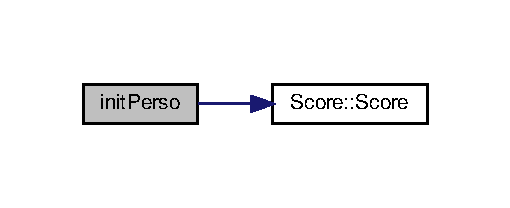
\includegraphics[width=245pt]{PP_8h_a06d4dad62654fc7399c91ef52e319c3c_cgraph}
\end{center}
\end{figure}
Here is the caller graph for this function\+:\nopagebreak
\begin{figure}[H]
\begin{center}
\leavevmode
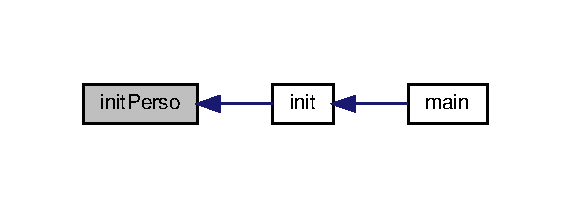
\includegraphics[width=274pt]{PP_8h_a06d4dad62654fc7399c91ef52e319c3c_icgraph}
\end{center}
\end{figure}
\mbox{\Hypertarget{PP_8h_a9e39e2d357f18982e3ec80e8ee8e2401}\label{PP_8h_a9e39e2d357f18982e3ec80e8ee8e2401}} 
\index{P\+P.\+h@{P\+P.\+h}!mouvement\+\_\+personnage@{mouvement\+\_\+personnage}}
\index{mouvement\+\_\+personnage@{mouvement\+\_\+personnage}!P\+P.\+h@{P\+P.\+h}}
\subsubsection{\texorpdfstring{mouvement\+\_\+personnage()}{mouvement\_personnage()}}
{\footnotesize\ttfamily void mouvement\+\_\+personnage (\begin{DoxyParamCaption}\item[{\hyperlink{structPersonnage__Principal}{Personnage\+\_\+\+Principal}}]{tab\+\_\+p\mbox{[}$\,$\mbox{]},  }\item[{S\+D\+L\+\_\+\+Surface $\ast$}]{screen,  }\item[{S\+D\+L\+\_\+\+Surface $\ast$}]{background,  }\item[{S\+D\+L\+\_\+\+Rect}]{position\+\_\+bakcground,  }\item[{int}]{mode }\end{DoxyParamCaption})}



pour faire le controle du personnage. 


\begin{DoxyParams}{Parameters}
{\em tab\+\_\+p} & un tableau de 2 personnage \\
\hline
{\em screen} & variable S\+D\+L\+\_\+\+Surface de l\textquotesingle{}ecran \\
\hline
{\em background} & variable S\+D\+L\+\_\+\+Surface du background \\
\hline
{\em position\+\_\+bakcground} & variable S\+D\+L\+\_\+\+Rect de la position du background \\
\hline
{\em mode} & 0 pour le mode singleplayer et 1 pour le mode multiplayer \\
\hline
\end{DoxyParams}
\begin{DoxyReturn}{Returns}
Nothing 
\end{DoxyReturn}
Here is the call graph for this function\+:\nopagebreak
\begin{figure}[H]
\begin{center}
\leavevmode
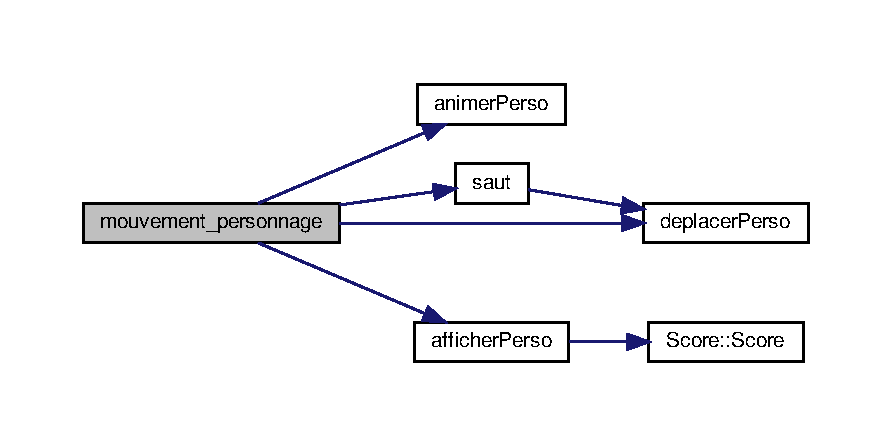
\includegraphics[width=350pt]{PP_8h_a9e39e2d357f18982e3ec80e8ee8e2401_cgraph}
\end{center}
\end{figure}
Here is the caller graph for this function\+:\nopagebreak
\begin{figure}[H]
\begin{center}
\leavevmode
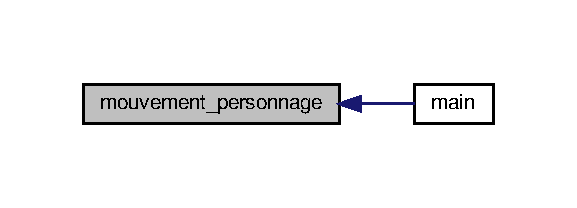
\includegraphics[width=277pt]{PP_8h_a9e39e2d357f18982e3ec80e8ee8e2401_icgraph}
\end{center}
\end{figure}
\mbox{\Hypertarget{PP_8h_a3fe04c57396598b16d78bd4065a8824d}\label{PP_8h_a3fe04c57396598b16d78bd4065a8824d}} 
\index{P\+P.\+h@{P\+P.\+h}!remis\+\_\+a\+\_\+zero@{remis\+\_\+a\+\_\+zero}}
\index{remis\+\_\+a\+\_\+zero@{remis\+\_\+a\+\_\+zero}!P\+P.\+h@{P\+P.\+h}}
\subsubsection{\texorpdfstring{remis\+\_\+a\+\_\+zero()}{remis\_a\_zero()}}
{\footnotesize\ttfamily void remis\+\_\+a\+\_\+zero (\begin{DoxyParamCaption}\item[{\hyperlink{structPersonnage__Principal}{Personnage\+\_\+\+Principal}}]{tab\+\_\+p\mbox{[}$\,$\mbox{]},  }\item[{int}]{mode }\end{DoxyParamCaption})}



pour remettre a zero tout les paramettre du jeu apres boucle de jeu. 


\begin{DoxyParams}{Parameters}
{\em tab\+\_\+p} & un tableau de 2 personnage \\
\hline
{\em mode} & 0 pour le mode singleplayer et 1 pour le mode multiplayer \\
\hline
\end{DoxyParams}
\begin{DoxyReturn}{Returns}
Nothing 
\end{DoxyReturn}
Here is the caller graph for this function\+:\nopagebreak
\begin{figure}[H]
\begin{center}
\leavevmode
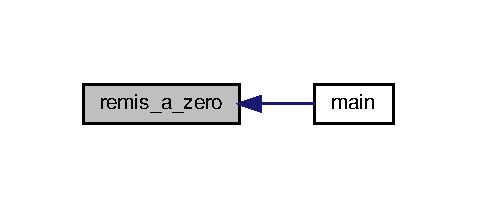
\includegraphics[width=229pt]{PP_8h_a3fe04c57396598b16d78bd4065a8824d_icgraph}
\end{center}
\end{figure}
\mbox{\Hypertarget{PP_8h_a23102f7e1f31031abb303525289bfb37}\label{PP_8h_a23102f7e1f31031abb303525289bfb37}} 
\index{P\+P.\+h@{P\+P.\+h}!saut@{saut}}
\index{saut@{saut}!P\+P.\+h@{P\+P.\+h}}
\subsubsection{\texorpdfstring{saut()}{saut()}}
{\footnotesize\ttfamily void saut (\begin{DoxyParamCaption}\item[{\hyperlink{structPersonnage__Principal}{Personnage\+\_\+\+Principal} $\ast$}]{p }\end{DoxyParamCaption})}



pour faire sauter le peronnage ( cette fonction est faite pour un saut de 5 frame ). 


\begin{DoxyParams}{Parameters}
{\em p} & la variable du personnage \\
\hline
\end{DoxyParams}
\begin{DoxyReturn}{Returns}
Nothing 
\end{DoxyReturn}
Here is the call graph for this function\+:\nopagebreak
\begin{figure}[H]
\begin{center}
\leavevmode
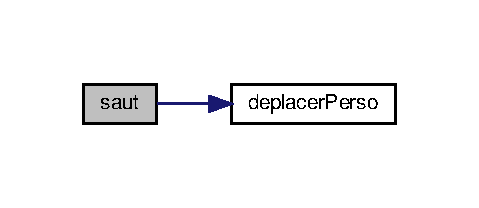
\includegraphics[width=230pt]{PP_8h_a23102f7e1f31031abb303525289bfb37_cgraph}
\end{center}
\end{figure}
Here is the caller graph for this function\+:\nopagebreak
\begin{figure}[H]
\begin{center}
\leavevmode
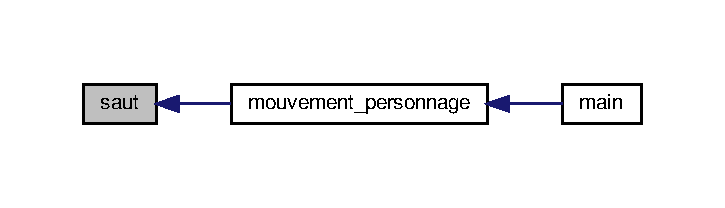
\includegraphics[width=348pt]{PP_8h_a23102f7e1f31031abb303525289bfb37_icgraph}
\end{center}
\end{figure}

%--- End generated contents ---

% Index
\backmatter
\newpage
\phantomsection
\clearemptydoublepage
\addcontentsline{toc}{chapter}{Index}
\printindex

\end{document}
